% Wednesday 1.24
\begin{theorem}
Every planar graph has a Pfaffian orientation.
\end{theorem}
\begin{theorem}[EDIT: Kuratowski]
A graph is planar if and only if there is no subdivision isomorphic to $K_{3,3}$ or $K_5$.
\end{theorem}
\begin{theorem}
A graph has a Pfaffian orientation if and only if no $K_{3,3}$.
\end{theorem}
\begin{theorem}
The number of pilings using dominos on an $m\times n$ board is 
$$T(m,n)=\prod_{j=1}^{m}\prod_{k=1}^n(4\cos^2(\frac{\pi j}{m+1})+4\cos^2(\frac{\pi k}{n+1}))^{\frac{1}{4}}.$$
\end{theorem}
\begin{proof}
Any two domino tilings are related by a sequence of flips.
\begin{figure}[h!]
\centering
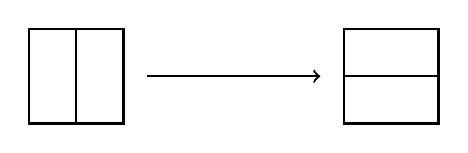
\begin{tikzpicture}[baseline=(current bounding box.center)]
    \pgfmathsetmacro{\r}{0.60};
    \foreach \x in {0,...,2}{
    \foreach \y in {0,...,2}{
    \node[inner sep=0](v\x\y)at(\r*\x,\r*\y){};}}
    \draw[thick](v00.center)--(v20.center)--(v22.center)--(v02.center)--cycle;
    \path[thick](v10.center)edge(v12.center);
    \draw[thick,->] (1.5,0.6) -- (3.7,0.6);
  \begin{scope}[xshift=4cm]
    \foreach \x in {0,...,2}{
    \foreach \y in {0,...,2}{
    \node[inner sep=0](v\x\y)at(\r*\x,\r*\y){};}}
    \draw[thick](v00.center)--(v20.center)--(v22.center)--(v02.center)--cycle;
    \path[thick](v01.center)edge(v21.center);
  \end{scope}
\end{tikzpicture}
\label{fig:domino_flip}
\caption{Flip}
\end{figure}
Any two perfect matchings contribute to the same sgn. Thus the number of perfect matchings of $P_m\square P_n$ is $|Pf(\vec{A}(D))|=\sqrt{|\det(\vec{A}(G))|}$. By rescaling you get $|\det(A)|=|\det(A'')|$, where 
$$A''=I_m\otimes A(P_n)-i(A(P_m)\otimes I_n).$$
Recall that the eigenvalues of $P_n$ are $2\cos(\frac{\pi k}{n+1}),k\in[n]$. Therefore, eigenvalues of $A''$ are 
$$2\cos(\frac{\pi k}{n+1})-i2\cos(\frac{\pi j}{m+1}).$$
Then we have the number of perfect matchings 
\begin{align*}
&|Pf(\vec{A}(D))|=\sqrt{|\det(A)|}\\
=&|\det(A'')|^{\frac{1}{2}}\\
=&\prod_{j=1}^{m}\prod_{k=1}^n |2\cos(\dfrac{\pi k}{n+1}) - i 2\cos(\dfrac{\pi k}{n+1})|^{1/4}
\end{align*}


\end{proof}

\subsection{Asymptotic of $T(m,n)$}
We have
\begin{align*}
\dfrac{\log (T(m,n))}{mn} &= \dfrac{1}{mn} \log \prod_{j=1}^{m}\prod_{k=1}^n(4\cos^2(\frac{\pi j}{m+1})+4\cos^2(\frac{\pi k}{n+1}))^{\frac{1}{4}}\\
&=\dfrac{1}{4\pi^2}(\dfrac{\pi}{m})(\dfrac{\pi}{n})\sum\limits_{j=1}^m\sum_{k=1}^n\log (4\cos^2(\dfrac{\pi j}{m+1})+4\cos^2(\dfrac{\pi k}{n+1}))\\
\xrightarrow{m,n \rightarrow \infty}&=\dfrac{1}{4\pi^2}\int_0^{\pi}\int_0^{\pi}\log(4\cos ^2x+4\cos^2y)\mathrm{d}x \mathrm{d}y\\
&=\dfrac{G}{\pi}
\end{align*}
where $G = \dfrac{1}{4\pi}\int_0^{\pi}\int_0^{\pi}\log(4\cos ^2x+4\cos^2y)\mathrm{d}x \mathrm{d}y=1-\dfrac{1}{3^2}+\dfrac{1}{5^2}+...$

(Open Problem) is G irrational?

$\log T(m,n) \approx G_{m,n}$. So $T(m,n) \approx \mathrm{e}^{G_{m,n}/\pi}$

